%% abtex2-modelo-include-comandos.tex, v-1.9.6 laurocesar
%% Copyright 2012-2016 by abnTeX2 group at http://www.abntex.net.br/ 
%%
%% This work may be distributed and/or modified under the
%% conditions of the LaTeX Project Public License, either version 1.3
%% of this license or (at your option) any later version.
%% The latest version of this license is in
%%   http://www.latex-project.org/lppl.txt
%% and version 1.3 or later is part of all distributions of LaTeX
%% version 2005/12/01 or later.
%%
%% This work has the LPPL maintenance status `maintained'.
%% 
%% The Current Maintainer of this work is the abnTeX2 team, led
%% by Lauro César Araujo. Further information are available on 
%% http://www.abntex.net.br/
%%
%% This work consists of the files abntex2-modelo-include-comandos.tex
%% and abntex2-modelo-img-marca.pdf
%%

% ---
% Este capítulo, utilizado por diferentes exemplos do abnTeX2, ilustra o uso de
% comandos do abnTeX2 e de LaTeX.
% ---

% ---
% TABELAS
% ---
\makeatletter
\renewcommand{\IBGEtab}[3]{%
	\savebox{\myptabbox}{{\ABNTEXfontereduzida #2}}%
	\settowidth{\myptabboxwidth}{\usebox{\myptabbox}}%
	\centering%
	\parbox{\myptabboxwidth}{%
		\configurecaptions
		#1%
		{\ABNTEXfontereduzida%
			#2%
		}%
		#3}%
}

\chapter{Resultados de comandos}\label{cap_exemplos}


% ---
\section{Codificação dos arquivos: UTF8}
% ---

A codificação de todos os arquivos do \abnTeX\ é \texttt{UTF8}. É necessário que
você utilize a mesma codificação nos documentos que escrever, inclusive nos
arquivos de base bibliográficas |.bib|.

% ---
\section{Citações diretas}
\label{sec-citacao}
% ---

\index{citações!diretas}Utilize o ambiente \texttt{citacao} para incluir
citações diretas com mais de três linhas:

\begin{citacao}
As citações diretas, no texto, com mais de três linhas, devem ser
destacadas com recuo de 4 cm da margem esquerda, com letra menor que a do texto
utilizado e sem as aspas. No caso de documentos datilografados, deve-se
observar apenas o recuo \cite{NBR10520:2002}.
\end{citacao}

Use o ambiente assim:

\begin{verbatim}
\begin{citacao}
As citações diretas, no texto, com mais de três linhas [...] deve-se
observar apenas o recuo \cite{NBR10520:2002}.
\end{citacao}
\end{verbatim}

O ambiente \texttt{citacao} pode receber como parâmetro opcional um nome de
idioma previamente carregado nas opções da classe (\autoref{sec-hifenizacao}). Nesse
caso, o texto da citação é automaticamente escrito em itálico e a hifenização é
ajustada para o idioma selecionado na opção do ambiente. Por exemplo:

\begin{verbatim}
\begin{citacao}[english]
Text in English language in italic with correct hyphenation.
\end{citacao}
\end{verbatim}

Tem como resultado:

\begin{citacao}[english]
Text in English language in italic with correct hyphenation.
\end{citacao}

\index{citações!simples}Citações simples, com até três linhas, devem ser
incluídas com aspas. Observe que em \LaTeX as aspas iniciais são diferentes das
finais: ``Amor é fogo que arde sem se ver''.

% ---
\section{Notas de rodapé}
% ---

As notas de rodapé são detalhadas pela NBR 14724:2011 na seção 5.2.1\footnote{As
notas devem ser digitadas ou datilografadas dentro das margens, ficando
separadas do texto por um espaço simples de entre as linhas e por filete de 5
cm, a partir da margem esquerda. Devem ser alinhadas, a partir da segunda linha
da mesma nota, abaixo da primeira letra da primeira palavra, de forma a destacar
o expoente, sem espaço entre elas e com fonte menor
\textcite{NBR14724:2011}.}\footnote{Caso uma série de notas sejam
criadas sequencialmente, o \abnTeX\ instrui o \LaTeX\ para que uma vírgula seja
colocada após cada número do expoente que indica a nota de rodapé no corpo do
texto.}\footnote{Verifique se os números do expoente possuem uma vírgula para
dividi-los no corpo do texto.}. 


% ---
\section{Tabelas}
% ---
\index{tabelas}A \autoref{tab-nivinv} é um exemplo de tabela construída em
\LaTeX.

\begin{table}[htb]
	\ABNTEXfontereduzida
	\caption[Níveis de investigação]{Níveis de investigação.}
	\label{tab-nivinv}
	\begin{tabular}{p{2.6cm} p{6.0cm} p{2.25cm} p{3.40cm}}
		\toprule
		\textbf{Nível de Investigação} & \textbf{Insumos}  & \textbf{Sistemas de Investigação}  & \textbf{Produtos}  \\
		\midrule
		Meta-nível & Filosofia\index{filosofia} da Ciência  & Epistemologia &
		Paradigma  \\
		
		Nível do objeto & Paradigmas do metanível e evidências do nível inferior &
		Ciência  & Teorias e modelos \\
		
		Nível inferior & Modelos e métodos do nível do objeto e problemas do nível inferior & Prática & Solução de problemas  \\
		\bottomrule
	\end{tabular}
	\ABNTEXfontereduzida\legend{Fonte: \textcite{van86}}
\end{table}

Já a \autoref{tabela-ibge} apresenta uma tabela criada conforme o padrão do
\textcite{ibge1993} requerido pelas normas da ABNT para documentos técnicos e
acadêmicos.

\begin{table}[htb]

\IBGEtab{%
  \caption{Um Exemplo de tabela alinhada que pode ser longa
  ou curta, conforme padrão IBGE.}%
  \label{tabela-ibge}
	}{%
	  \begin{tabular}{ccc}
	  \toprule
	   Nome & Nascimento & Documento \\
	  \midrule
	   Maria da Silva & 11/11/1111 & 111.111.111-11 \\
	   
	   João Souza & 11/11/2111 & 211.111.111-11 \\
	   
	   Laura Vicuña & 05/04/1891 & 3111.111.111-11 \\
	  \bottomrule
	\end{tabular}%
	}{%
	\fonte{Produzido pelos autores.}%
	\nota{Esta é uma nota, que diz que os dados são baseados na regressão linear.}%
	\nota[Anotações]{Uma anotação adicional, que pode ser seguida de várias outras.}%
  }
\end{table}

\section{Uso de Tabelas com multi colunas}

\begin{table}[htb]
	\IBGEtab{%
		\caption{Desempenho da \textit{Stack} sem o uso do \textit{Varnish} cache}%
		\label{tab:teste-sem-varnish}
	}{%
		\begin{tabular}{lcccccc}
			\toprule
			\multicolumn{1}{c}{\multirow{3}{*}{Tipo de Conteúdo}} & \multicolumn{6}{c}{Conexões concorrentes}                         \\ \cline{2-7}
			\multicolumn{1}{c}{}                                  & \multicolumn{2}{c}{1} & \multicolumn{2}{c}{10} & 100     &       \\ \cline{2-7}
			\multicolumn{1}{c}{}                                  & Req/Seg    & Tempo     & Req/Seg     & Tempo     & Req/Seg & Tempo \\ \hline
			Página inicial                                          & 250,14     & 3,998     & 663,09      & 1,508     & 625,4   & 1,599 \\
			Notícia com foto - 40,44 KB                             & 169,89     & 5,079     & 494,43      & 2,023     & 466,33  & 2,144 \\
			Página comum - 37,74 KB                                 & 195,96     & 5,103     & 503,99      & 1,984     & 463,09  & 2,159 \\
			Imagem - 108 KB                                         & 8,72       & 114,676   & 26,75       & 37,377    & 624,56  & 1,601 \\
			Arquivo de CSS - 1,42 KB                                & 296,49     & 3,373     & 798,21      & 1,253     & 757,9   & 1,319 \\ \bottomrule
		\end{tabular}
	}{%
		\fonte{Autor}%
	}
\end{table}

A \autoref{tab:teste-com-varnish} apresenta os resultados dos testes na composição com o \textit{Varnish}.


Tabelas exibem dados numéricos que podem ser facilmente comparados.

\begin{table}[htb]
	\IBGEtab{%
		\caption{Desempenho da \textit{Stack} com o uso do \textit{Varnish} cache}%
		\label{tab:teste-com-varnish}
	}{%
		\begin{tabular}{lcccccc}
			\toprule
			\multicolumn{1}{c}{\multirow{3}{*}{Tipo de Conteúdo}} & \multicolumn{6}{c}{Conexões concorrentes}                         \\ \cline{2-7}
			\multicolumn{1}{c}{}                                  & \multicolumn{2}{c}{1} & \multicolumn{2}{c}{10} & 100     &       \\ \cline{2-7}
			\multicolumn{1}{c}{}                                  & Req/Seg    & Tempo     & Req/Seg     & Tempo     & Req/Seg & Tempo \\ \hline
			Página inicial              & 20611,76 & 0,049 & 58664,79 & 0,017 & 53504,26 & 0,019 \\
			Notícia com foto - 40,44 KB & 18289,06 & 0,055 & 49504,22 & 0,02  & 55116,46 & 0,018 \\
			Página comum - 37,74 KB     & 18542,42 & 0,054 & 47876,21 & 0,021 & 55802,01 & 0,018 \\
			Imagem - 108 KB             & 17445,28 & 0,057 & 52603,62 & 0,019 & 52833,74 & 0,019 \\
			Arquivo de CSS - 1,42 KB    & 17107,97 & 0,058 & 58702,67 & 0,017 & 51502,59 & 0,019 \\ \bottomrule
		\end{tabular}
	}{%
		\fonte{Autor}%
	}
\end{table}

% ---
\section{Quadros}
% ---

\subsection{Quadro simples}

Uso de quadros, que se diferenciam das tabelas por conter mais informações do tipo descritivas e não uma compilação de números e informações, como seria se fosse uma tabela.


\begin{quadro}
	\caption{\label{q:artefatos-imp}Artefato produzido na fase de implementação}
	\resizebox{\textwidth}{!}{%
		\begin{tabular}{|p{3.0cm}|c|p{12.0cm}|c|}
			\hline
			Nome & Sigla & Descrição & Tarefa \\ \hline
			Relatório Final & RelFn & Refinamento do Relatório de Demandas (RelDm), sendo incluídas as alterações realizadas durante a fase de desenvolvimento {[}caso houver{]} e inserção de conteúdo do sítio. Ele deverá conter toda a estrutura final do sítio, incluindo a forma de distribuição de arquivos e padronização de nomes e metadados para classificação das informações. & I-7 \\ \hline
		\end{tabular}%
	}
	\legend{Fonte: Autor}
\end{quadro}

\subsection{Quadro redimensionado quando é muito grande.}\label{ap:benchmark_cms}
% ---
\begin{quadro}[htb]
	\caption{\label{q:sgc_universidades}Quadro sobre pesquisa sobre uso de SGCs e adoção da IDG pelas Universidades Públicas Federais}
	\resizebox{\textwidth}{!}{%
		\begin{tabular}{|l|l|c|c|}
			\hline
			Nome da Instituição                                                            & \multicolumn{1}{c|}{URL}          & SGC       & Usa a IDG? \\ \hline
			FUNDAÇÃO UNIVERSIDADE FEDERAL DA GRANDE DOURADOS (UFGD)                        & http://portal.ufgd.edu.br         & Outros    & Não           \\ \hline
			FUNDAÇÃO UNIVERSIDADE FEDERAL DE CIÊNCIAS DA SAÚDE DE PORTO ALEGRE (UFCSPA)    & http://www.ufcspa.edu.br          & Joomla    & Não           \\ \hline
			FUNDAÇÃO UNIVERSIDADE FEDERAL DE RONDÔNIA (UNIR)                               & http://www.unir.br                & Outros    & Não           \\ \hline
			FUNDAÇÃO UNIVERSIDADE FEDERAL DO ABC (UFABC)                                   & http://www.ufabc.edu.br           & Joomla    & Sim           \\ \hline
			FUNDAÇÃO UNIVERSIDADE FEDERAL DO PAMPA - UNIPAMPA (UNIPAMPA)                   & http://novoportal.unipampa.edu.br & Drupal    & Não           \\ \hline
			FUNDAÇÃO UNIVERSIDADE FEDERAL DO TOCANTINS (UFT)                               & http://ww2.uft.edu.br             & Joomla    & Sim           \\ \hline
			FUNDAÇÃO UNIVERSIDADE FEDERAL DO VALE DO SÃO FRANCISCO (UNIVASF)               & http://portais.univasf.edu.br     & Plone     & Sim           \\ \hline
			UNIVERSIDADE DA INTEGRAÇÃO INTERNACIONAL DA LUSOFONIA AFRO-BRASILEIRA (UNILAB) & http://www.unilab.edu.br          & Wordpress & Não           \\ \hline
			UNIVERSIDADE DE BRASÍLIA (UNB)                                                 & http://www.unb.br                 & Joomla    & Não           \\ \hline
			UNIVERSIDADE FEDERAL DA BAHIA (UFBA)                                           & http://www.ufba.br                & Drupal    & Não           \\ \hline
			UNIVERSIDADE FEDERAL DA FRONTEIRA SUL (UFFS)                                   & http://www.uffs.edu.br            & Plone     & Não           \\ \hline
			UNIVERSIDADE FEDERAL DA INTEGRAÇÃO LATINO-AMERICANA (UNILA)                    & http://www.unila.edu.br           & Drupal    & Não           \\ \hline
			UNIVERSIDADE FEDERAL DA PARAÍBA (UFPB)                                         & http://www.ufpb.br                & Drupal    & Não           \\ \hline
			UNIVERSIDADE FEDERAL DE ALAGOAS (UFAL)                                         & http://www.ufal.edu.br            & Plone     & Não           \\ \hline
			UNIVERSIDADE FEDERAL DE ALFENAS (UNIFAL-MG)                                    & http://www.unifal-mg.edu.br       & Outros    & Não           \\ \hline
			UNIVERSIDADE FEDERAL DE CAMPINA GRANDE (UFCG)                                  & http://www.ufcg.edu.br            & Outros    & Não           \\ \hline
			UNIVERSIDADE FEDERAL DE GOIÁS (UFG)                                            & http://www.ufg.br                 & Outros    & Não           \\ \hline
			UNIVERSIDADE FEDERAL DE ITAJUBÁ - UNIFEI (UNIFEI)                              & https://www.unifei.edu.br/        & Drupal    & Não           \\ \hline
			UNIVERSIDADE FEDERAL DE JUIZ DE FORA (UFJF)                                    & http://www.ufjf.br                & Outros    & Não           \\ \hline
			UNIVERSIDADE FEDERAL DE LAVRAS (UFLA)                                          & http://www.ufla.br                & Wordpress & Não           \\ \hline
			UNIVERSIDADE FEDERAL DE MATO GROSSO (UFMT)                                     & http://www.ufmt.br                & Outros    & Não           \\ \hline
			UNIVERSIDADE FEDERAL DE MATO GROSSO DO SUL (UFMS)                              & http://www.ufms.br                & Wordpress & Não           \\ \hline
			UNIVERSIDADE FEDERAL DE MINAS GERAIS (UFMG)                                    & http://www.ufmg.br                & Outros    & Não           \\ \hline
			UNIVERSIDADE FEDERAL DE OURO PRETO (UFOP)                                      & http://www.ufop.br                & Drupal    & Não           \\ \hline
			UNIVERSIDADE FEDERAL DE PELOTAS (UFPEL)                                        & http://portal.ufpel.edu.br        & Wordpress & Não           \\ \hline
			UNIVERSIDADE FEDERAL DE PERNAMBUCO (UFPE)                                      & http://www.ufpe.br                & Joomla    & Não           \\ \hline
			UNIVERSIDADE FEDERAL DE RORAIMA (UFRR)                                         & http://ufrr.br                    & Joomla    & Sim           \\ \hline
			UNIVERSIDADE FEDERAL DE SANTA CATARINA (UFSC)                                  & http://ufsc.br                    & Wordpress & Sim           \\ \hline
			UNIVERSIDADE FEDERAL DE SANTA MARIA (UFSM)                                     & http://site.ufsm.br               & Outros    & Não           \\ \hline
			UNIVERSIDADE FEDERAL DE SÃO CARLOS (UFSCAR)                                    & http://www2.ufscar.br             & Plone     & Não           \\ \hline
			UNIVERSIDADE FEDERAL DE SÃO JOÃO DEL REI (UFSJ)                                & http://www.ufsj.edu.br            & Outros    & Não           \\ \hline
			UNIVERSIDADE FEDERAL DE SÃO PAULO (UNIFESP)                                    & http://www.unifesp.br             & Joomla    & Não           \\ \hline
			UNIVERSIDADE FEDERAL DE SERGIPE (UFS)                                          & http://www.ufs.br                 & Outros    & Não           \\ \hline
			UNIVERSIDADE FEDERAL DE UBERLÂNDIA (UFU)                                       & http://www.ufu.br                 & Drupal    & Sim           \\ \hline
			UNIVERSIDADE FEDERAL DE VIÇOSA (UFV)                                           & http://www.ufv.br                 & Wordpress & Não           \\ \hline
			UNIVERSIDADE FEDERAL DO ACRE (UFAC)                                            & http://www.ufac.br                & Plone     & Sim           \\ \hline
			UNIVERSIDADE FEDERAL DO AMAPÁ (UNIFAP)                                         & http://www.unifap.br              & Outros    & Não           \\ \hline
			UNIVERSIDADE FEDERAL DO AMAZONAS (UFAM)                                        & http://ufam.edu.br                & Joomla    & Não           \\ \hline
			UNIVERSIDADE FEDERAL DO CARIRI (UFCA)                                          & http://www.ufca.edu.br            & Joomla    & Não           \\ \hline
			UNIVERSIDADE FEDERAL DO CEARÁ (UFC)                                            & http://www.ufc.br                 & Joomla    & Não           \\ \hline
			UNIVERSIDADE FEDERAL DO ESPÍRITO SANTO (UFES)                                  & http://www.ufes.br                & Drupal    & Não           \\ \hline
			UNIVERSIDADE FEDERAL DO ESTADO DO RIO DE JANEIRO (UNIRIO)                      & http://www.unirio.br              & Plone     & Não           \\ \hline
			UNIVERSIDADE FEDERAL DO MARANHÃO (UFMA)                                        & http://portais.ufma.br            & Outros    & Sim           \\ \hline
			UNIVERSIDADE FEDERAL DO OESTE DA BAHIA (UFOB)                                  & http://ufob.edu.br                & Joomla    & Não           \\ \hline
			UNIVERSIDADE FEDERAL DO OESTE DO PARÁ (UFOPA)                                  & http://www.ufopa.edu.br           & Plone     & Não           \\ \hline
			UNIVERSIDADE FEDERAL DO PARÁ (UFPA)                                            & http://portal.ufpa.br             & Outros    & Não           \\ \hline
			UNIVERSIDADE FEDERAL DO PARANÁ (UFPR)                                          & http://www.ufpr.br                & Wordpress & Não           \\ \hline
			UNIVERSIDADE FEDERAL DO PIAUÍ (UFPI)                                           & http://www.ufpi.br                & Joomla    & Sim           \\ \hline
			UNIVERSIDADE FEDERAL DO RECÔNCAVO DA BAHIA (UFRB)                              & http://ufrb.edu.br                & Joomla    & Sim           \\ \hline
			UNIVERSIDADE FEDERAL DO RIO DE JANEIRO (UFRJ)                                  & http://ufrj.br/                   & Drupal    & Não           \\ \hline
			UNIVERSIDADE FEDERAL DO RIO GRANDE (FURG)                                      & http://www.furg.br                & Outros    & Não           \\ \hline
			UNIVERSIDADE FEDERAL DO RIO GRANDE DO NORTE (UFRN)                             & http://www.ufrn.br                & Wordpress & Não           \\ \hline
			UNIVERSIDADE FEDERAL DO RIO GRANDE DO SUL (UFRGS)                              & http://www.ufrgs.br               & Plone     & Não           \\ \hline
			UNIVERSIDADE FEDERAL DO SUL DA BAHIA (UFESBA)                                  & http://www.ufsb.edu.br            & Wordpress & Não           \\ \hline
			UNIVERSIDADE FEDERAL DO SUL E SUDESTE DO PARÁ (UNIFESSPA)                      & http://www.unifesspa.edu.br       & Joomla    & Sim           \\ \hline
			UNIVERSIDADE FEDERAL DO TRIÂNGULO MINEIRO (UFTM)                               & http://www.uftm.edu.br            & Joomla    & Não           \\ \hline
			UNIVERSIDADE FEDERAL DOS VALES DO JEQUITINHONHA E MUCURI (UFVJM)               & http://www.ufvjm.edu.br           & Joomla    & Não           \\ \hline
			UNIVERSIDADE FEDERAL FLUMINENSE (UFF)                                          & http://www.uff.br                 & Drupal    & Não           \\ \hline
			UNIVERSIDADE FEDERAL RURAL DA AMAZÔNIA (UFRA)                                  & http://novo.ufra.edu.br           & Joomla    & Sim           \\ \hline
			UNIVERSIDADE FEDERAL RURAL DE PERNAMBUCO (UFRPE)                               & http://www.ufrpe.br               & Drupal    & Não           \\ \hline
			UNIVERSIDADE FEDERAL RURAL DO RIO DE JANEIRO (UFRRJ)                           & http://portal.ufrrj.br            & Wordpress & Não           \\ \hline
			UNIVERSIDADE FEDERAL RURAL DO SEMI-ÁRIDO (UFERSA)                              & http://ufersa.edu.br              & Wordpress & Não           \\ \hline
			UNIVERSIDADE TECNOLÓGICA FEDERAL DO PARANÁ (UTFPR)                             & http://www.utfpr.edu.br           & Plone     & Não           \\ \hline
		\end{tabular}
	}
	\legend{Fonte: Autor}
	\legend{Nota: pesquisa realizada em 16/03/2017 verificando os sites das próprias universidades.}
\end{quadro}

\clearpage 
% ---
\section{Códigos fonte}
% ---

\subsection{Código fonte do projeto Plone.IDG}\label{ap:cod-ploneidg}

Exemplo de representação de códigos no seu trabalho.

\begin{lstlisting}[caption={\textit{Dockerfile} modificada com alterações realizadas para implementar o \textit{Plone} na UFVJM},label={cod:plonedocker-mod}]
FROM plone:4.3

MAINTAINER Elias Alves <elias.alves@ufvjm.edu.br>

ARG BUILD_DATE
ARG VCS_REF

LABEL Name="Plone v4.3 IDG" \
Version="1.1.5.3" \
Architecture="x86_64" \
Dockerfile_location="/root/buildinfo" \
org.label-schema.build-date=$BUILD_DATE \
org.label-schema.name="Plone v4.3 IDG" \
org.label-schema.description="Modelo Plone v4.3 IDG escrito para implementacao no Portal da UFVJM" \
org.label-schema.url="http://portal.ufvjm.edu.br/" \
org.label-schema.vcs-ref=$VCS_REF \
org.label-schema.vcs-url="https://github.com/unixelias/plone.idg" \
org.label-schema.vendor="Elias Alves at UFVJM" \
org.label-schema.version="1.1.5" \
org.label-schema.version="1.1.5.3" \
org.label-schema.version="stable" \
org.label-schema.version="latest" \
org.label-schema.schema-version="1.0" \
org.label-schema.docker.cmd="docker run -p 8080:8080 -v ./data:/data unixelias/plone.idg"

USER plone
COPY site.cfg /plone/instance/

USER root
COPY Dockerfile /root/buildinfo

[...]

CMD ["start"]
\end{lstlisting}
\legend{Fonte: Autor}


\begin{lstlisting}[caption={\textit{site.cfg} modificado para instalar pacotes adicionais ao \textit{Plone} com IDG},label={cod:site-cfg-mod}]
[buildout]
extends =
buildout.cfg
https://raw.githubusercontent.com/unixelias/plone.idg/master/versions/1.1.5.3/versions.cfg
https://raw.githubusercontent.com/plonegovbr/portal.buildout/master/buildout.d/maintenance.cfg

[instance]
eggs +=
# Extensões mantidas pela comunidade PloneGov-BR
brasil.gov.portal
brasil.gov.facetada
brasil.gov.vlibrasnews
collective.opendata
# Extensões mantidas pelo Plone
plone.app.ldap
collective.lineage
collective.geo.bundle
collective.behavior.banner
collective.polls
Products.EasyNewsletter

[versions]
brasil.gov.portal = 1.1.5.1
\end{lstlisting}
\legend{Fonte: Autor}

\clearpage

\begin{lstlisting}[caption={\textit{versions.cfg} criado para pinar as versões dos pacotes adicionais a serem instalados no \textit{Plone} com a IDG},label={cod:versions-mod}]
[buildout]

versions = versions

[versions]
brasil.gov.facetada = 1.0b1
brasil.gov.vlibrasnews = 1.0b1
collective.opendata = 1.0a2
\end{lstlisting}
\legend{Fonte: Autor}


\begin{lstlisting}[caption={\textit{docker-compose.yml} modificado para adaptar a pilha de serviços \textit{Plone} para o ambiente de produção do Portal da UFVJM},label={cod:docker-compose-mod}]
version: "2"
services:
varnish:
hostname: 'varnish'
image: eeacms/varnish
restart: 'always'
depends_on:
- haproxy
ports:
- 8080:6081/tcp
environment:
- BACKENDS=haproxy
- BACKENDS_PORT=5000
- BACKENDS_PROBE_INTERVAL=3s
- BACKENDS_PROBE_THRESHOLD=2
- BACKENDS_PROBE_TIMEOUT=1s
- BACKENDS_PROBE_WINDOW=3
- DNS_ENABLED=true

haproxy:
image: eeacms/haproxy
restart: 'always'
depends_on:
- ploneidg
ports:
- 1936:1936
environment:
- BACKENDS=ploneidg
- BACKENDS_PORT=8080
- SERVICE_NAMES=ploneidg
- DNS_ENABLED=true
- STATS_AUTH=admin:admin

zeoserver:
hostname: 'zeoserver'
image: unixelias/plone.idg:latest
command:
- zeoserver
volumes:
- data:/data/filestorage
- data:/data/blobstorage
- data:/data/backups
- data:/data/blobstoragebackups

ploneidg:
image: unixelias/plone.idg:latest
depends_on:
- zeoserver
environment:
- ZEO_ADDRESS=zeoserver:8100

volumes:
data:
driver: local-persist
driver_opts:
mountpoint: /srv/portal/data
command: chown -R 500:500 /data
\end{lstlisting}
\legend{Fonte: Autor}

% ---
\section{Figuras}
% ---

\index{figuras}Figuras podem ser criadas diretamente em \LaTeX,
como o exemplo da \autoref{fig_circulo}.

\begin{figure}[htb]
	\caption{\label{fig_circulo}A delimitação do espaço}
	\begin{center}
	    \setlength{\unitlength}{5cm}
		\begin{picture}(1,1)
		\put(0,0){\line(0,1){1}}
		\put(0,0){\line(1,0){1}}
		\put(0,0){\line(1,1){1}}
		\put(0,0){\line(1,2){.5}}
		\put(0,0){\line(1,3){.3333}}
		\put(0,0){\line(1,4){.25}}
		\put(0,0){\line(1,5){.2}}
		\put(0,0){\line(1,6){.1667}}
		\put(0,0){\line(2,1){1}}
		\put(0,0){\line(2,3){.6667}}
		\put(0,0){\line(2,5){.4}}
		\put(0,0){\line(3,1){1}}
		\put(0,0){\line(3,2){1}}
		\put(0,0){\line(3,4){.75}}
		\put(0,0){\line(3,5){.6}}
		\put(0,0){\line(4,1){1}}
		\put(0,0){\line(4,3){1}}
		\put(0,0){\line(4,5){.8}}
		\put(0,0){\line(5,1){1}}
		\put(0,0){\line(5,2){1}}
		\put(0,0){\line(5,3){1}}
		\put(0,0){\line(5,4){1}}
		\put(0,0){\line(5,6){.8333}}
		\put(0,0){\line(6,1){1}}
		\put(0,0){\line(6,5){1}}
		\end{picture}
	\end{center}
	\legend{Fonte: os autores}
\end{figure}

Ou então figuras podem ser incorporadas de arquivos externos, como é o caso da
\autoref{fig_grafico}. Se a figura que ser incluída se tratar de um diagrama, um
gráfico ou uma ilustração que você mesmo produza, priorize o uso de imagens
vetoriais no formato PDF. Com isso, o tamanho do arquivo final do trabalho será
menor, e as imagens terão uma apresentação melhor, principalmente quando
impressas, uma vez que imagens vetorias são perfeitamente escaláveis para
qualquer dimensão. Nesse caso, se for utilizar o Microsoft Excel para produzir
gráficos, ou o Microsoft Word para produzir ilustrações, exporte-os como PDF e
os incorpore ao documento conforme o exemplo abaixo. No entanto, para manter a
coerência no uso de software livre (já que você está usando \LaTeX e \abnTeX),
teste a ferramenta \textsf{InkScape}\index{InkScape}
(\url{http://inkscape.org/}). Ela é uma excelente opção de código-livre para
produzir ilustrações vetoriais, similar ao CorelDraw\index{CorelDraw} ou ao Adobe
Illustrator\index{Adobe Illustrator}. De todo modo, caso não seja possível
utilizar arquivos de imagens como PDF, utilize qualquer outro formato, como
JPEG, GIF, BMP, etc. Nesse caso, você pode tentar aprimorar as imagens
incorporadas com o software livre \textsf{Gimp}\index{Gimp}
(\url{http://www.gimp.org/}). Ele é uma alternativa livre ao Adobe
Photoshop\index{Adobe Photoshop}.

\begin{figure}[htb]
	\caption{\label{fig_grafico}Gráfico produzido em Excel e salvo como PDF}
	\begin{center}
	    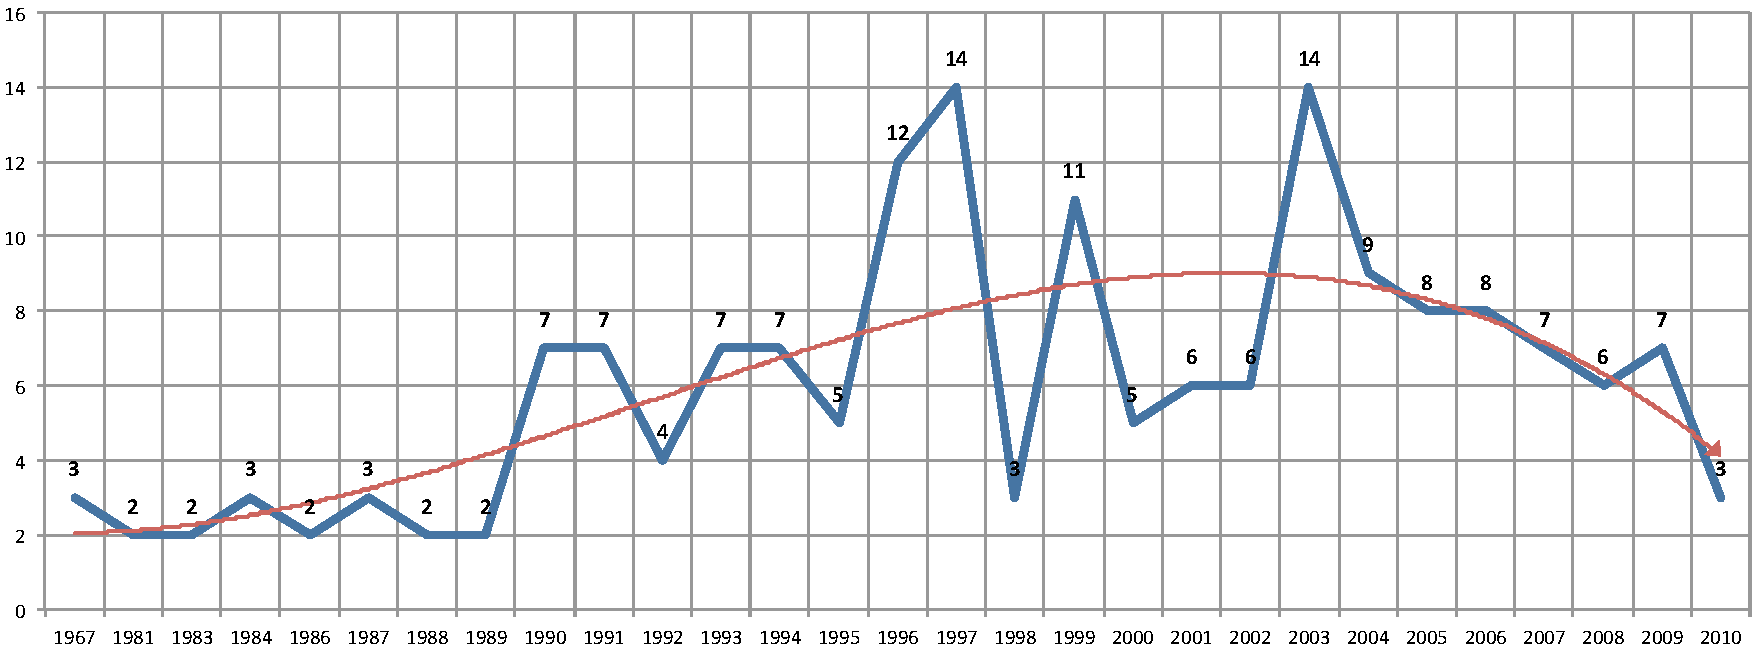
\includegraphics[scale=0.5]{img/abntex2-modelo-img-grafico.pdf}
	\end{center}
	\legend{Fonte: \textcite{araujo2012}}
\end{figure}

% ---
\subsection{Figuras em \emph{minipages}}
% ---

\emph{Minipages} são usadas para inserir textos ou outros elementos em quadros
com tamanhos e posições controladas. Veja o exemplo da
\autoref{fig_minipage_imagem1} e da \autoref{fig_minipage_grafico2}.

\begin{figure}[htb]
 \label{teste}
 \centering
  \begin{minipage}{0.4\textwidth}
    \centering
    \caption{Imagem 1 da minipage} \label{fig_minipage_imagem1}
    
\includegraphics[scale=0.9]{img/abntex2-modelo-img-marca.pdf}
    \legend{Fonte: Produzido pelos autores}
  \end{minipage}
  \hfill
  \begin{minipage}{0.4\textwidth}
    \centering
    \caption{Grafico 2 da minipage} \label{fig_minipage_grafico2}
    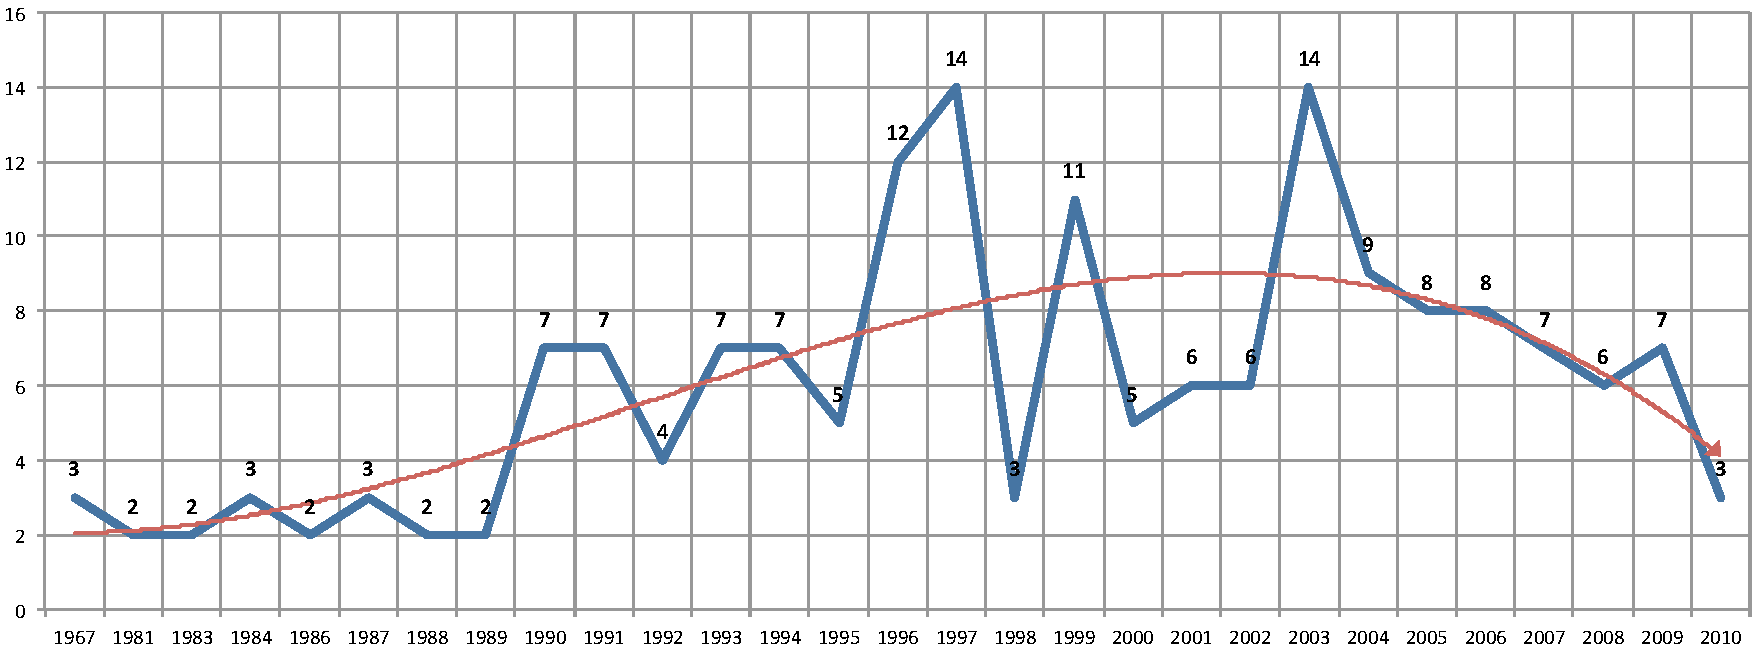
\includegraphics[scale=0.2]{img/abntex2-modelo-img-grafico.pdf}
    \legend{Fonte: \textcite{araujo2012}}
  \end{minipage}
\end{figure}

Observe que, segundo a \textcite{NBR14724:2011}, as
ilustrações devem sempre ter numeração contínua e única em todo o documento:

\begin{citacao}
Qualquer que seja o tipo de ilustração, sua identificação aparece na parte
superior, precedida da palavra designativa (desenho, esquema, fluxograma,
fotografia, gráfico, mapa, organograma, planta, quadro, retrato, figura,
imagem, entre outros), seguida de seu número de ordem de ocorrência no texto,
em algarismos arábicos, travessão e do respectivo título. Após a ilustração, na
parte inferior, indicar a fonte consultada (elemento obrigatório, mesmo que
seja produção do próprio autor), legenda, notas e outras informações
necessárias à sua compreensão (se houver). A ilustração deve ser citada no
texto e inserida o mais próximo possível do trecho a que se
refere. \cite{NBR14724:2011}
\end{citacao}

% ---
\section{Expressões matemáticas}
% ---

\index{expressões matemáticas}Use o ambiente \texttt{equation} para escrever
expressões matemáticas numeradas:

\begin{equation}
  \forall x \in X, \quad \exists \: y \leq \epsilon
\end{equation}

Escreva expressões matemáticas entre \$ e \$, como em $ \lim_{x \to \infty}
\exp(-x) = 0 $, para que fiquem na mesma linha.

\begin{equation}
	\left|\sum_{i=1}^n a_ib_i\right|
	\le
	\left(\sum_{i=1}^n a_i^2\right)^{1/2}
	\left(\sum_{i=1}^n b_i^2\right)^{1/2}
\end{equation}


Consulte mais informações sobre expressões matemáticas em
\url{https://github.com/abntex/abntex2/wiki/Referencias}.

% ---
\section{Enumerações: alíneas e subalíneas}
% ---

\index{alíneas}\index{subalíneas}\index{incisos}Quando for necessário enumerar
os diversos assuntos de uma seção que não possua título, esta deve ser
subdividida em alíneas \cite{NBR6024:2012}:

\begin{alineas}

  \item os diversos assuntos que não possuam título próprio, dentro de uma mesma
  seção, devem ser subdivididos em alíneas; 
  
  \item o texto que antecede as alíneas termina em dois pontos;
  \item as alíneas devem ser indicadas alfabeticamente, em letra minúscula,
  seguida de parêntese. Utilizam-se letras dobradas, quando esgotadas as
  letras do alfabeto;

  \item as letras indicativas das alíneas devem apresentar recuo em relação à
  margem esquerda;

  \item o texto da alínea deve começar por letra minúscula e terminar em
  ponto-e-vírgula, exceto a última alínea que termina em ponto final;

  \item o texto da alínea deve terminar em dois pontos, se houver subalínea;

  \item a segunda e as seguintes linhas do texto da alínea começa sob a
  primeira letra do texto da própria alínea;
  
  \item subalíneas \cite{NBR6024:2012} devem ser conforme as alíneas a
  seguir:

  \begin{alineas}
     \item as subalíneas devem começar por travessão seguido de espaço;

     \item as subalíneas devem apresentar recuo em relação à alínea;

     \item o texto da subalínea deve começar por letra minúscula e terminar em
     ponto-e-vírgula. A última subalínea deve terminar em ponto final, se não
     houver alínea subsequente;

     \item a segunda e as seguintes linhas do texto da subalínea começam sob a
     primeira letra do texto da própria subalínea.
  \end{alineas}
  
  \item no \abnTeX\ estão disponíveis os ambientes \texttt{incisos} e
  \texttt{subalineas}, que em suma são o mesmo que se criar outro nível de
  \texttt{alineas}, como nos exemplos à seguir:
  
  \begin{incisos}
    \item \textit{Um novo inciso em itálico};
  \end{incisos}
  
  \item Alínea em \textbf{negrito}:
  
  \begin{subalineas}
    \item \textit{Uma subalínea em itálico};
    \item \underline{\textit{Uma subalínea em itálico e sublinhado}}; 
  \end{subalineas}
  
  \item Última alínea com \emph{ênfase}.
  
\end{alineas}

% ---
\section{Espaçamento entre parágrafos e linhas}
% ---

\index{espaçamento!dos parágrafos}O tamanho do parágrafo, espaço entre a margem
e o início da frase do parágrafo, é definido por:

\begin{verbatim}
   \setlength{\parindent}{1.3cm}
\end{verbatim}

\index{espaçamento!do primeiro parágrafo}Por padrão, não há espaçamento no
primeiro parágrafo de cada início de divisão do documento
(\autoref{sec-divisoes}). Porém, você pode definir que o primeiro parágrafo
também seja indentado, como é o caso deste documento. Para isso, apenas inclua o
pacote \textsf{indentfirst} no preâmbulo do documento:

\begin{verbatim}
   \usepackage{indentfirst}      % Indenta o primeiro parágrafo de cada seção.
\end{verbatim}

\index{espaçamento!entre os parágrafos}O espaçamento entre um parágrafo e outro
pode ser controlado por meio do comando:

\begin{verbatim}
  \setlength{\parskip}{0.2cm}  % tente também \onelineskip
\end{verbatim}

\index{espaçamento!entre as linhas}O controle do espaçamento entre linhas é
definido por:

\begin{verbatim}
  \OnehalfSpacing       % espaçamento um e meio (padrão); 
  \DoubleSpacing        % espaçamento duplo
  \SingleSpacing        % espaçamento simples	
\end{verbatim}

Para isso, também estão disponíveis os ambientes:

\begin{verbatim}
  \begin{SingleSpace} ...\end{SingleSpace}
  \begin{Spacing}{hfactori} ... \end{Spacing}
  \begin{OnehalfSpace} ... \end{OnehalfSpace}
  \begin{OnehalfSpace*} ... \end{OnehalfSpace*}
  \begin{DoubleSpace} ... \end{DoubleSpace}
  \begin{DoubleSpace*} ... \end{DoubleSpace*} 
\end{verbatim}

Para mais informações, consulte \textcite{memoir}.

% ---
\section{Inclusão de outros arquivos}\label{sec-include}
% ---

É uma boa prática dividir o seu documento em diversos arquivos, e não
apenas escrever tudo em um único. Esse recurso foi utilizado neste
documento. Para incluir diferentes arquivos em um arquivo principal,
de modo que cada arquivo incluído fique em uma página diferente, utilize o
comando:

\begin{verbatim}
   \include{documento-a-ser-incluido}      % sem a extensão .tex
\end{verbatim}

Para incluir documentos sem quebra de páginas, utilize:

\begin{verbatim}
   \input{documento-a-ser-incluido}      % sem a extensão .tex
\end{verbatim}

% ---
\section{Compilar o documento \LaTeX}
% ---

Geralmente os editores \LaTeX, como o
TeXlipse\footnote{\url{http://texlipse.sourceforge.net/}}, o
Texmaker\footnote{\url{http://www.xm1math.net/texmaker/}}, entre outros,
compilam os documentos automaticamente, de modo que você não precisa se
preocupar com isso.

No entanto, você pode compilar os documentos \LaTeX usando os seguintes
comandos, que devem ser digitados no \emph{Prompt de Comandos} do Windows ou no
\emph{Terminal} do Mac ou do Linux:

\begin{verbatim}
   pdflatex ARQUIVO_PRINCIPAL.tex
   bibtex ARQUIVO_PRINCIPAL.aux
   makeindex ARQUIVO_PRINCIPAL.idx 
   makeindex ARQUIVO_PRINCIPAL.nlo -s nomencl.ist -o ARQUIVO_PRINCIPAL.nls
   pdflatex ARQUIVO_PRINCIPAL.tex
   pdflatex ARQUIVO_PRINCIPAL.tex
\end{verbatim}

% ---
\section{Remissões internas}
% ---

Ao nomear a \autoref{tab-nivinv} e a \autoref{fig_circulo}, apresentamos um
exemplo de remissão interna, que também pode ser feita quando indicamos o
\autoref{cap_exemplos}, que tem o nome \emph{\nameref{cap_exemplos}}. O número
do capítulo indicado é \ref{cap_exemplos}, que se inicia à
\autopageref{cap_exemplos}\footnote{O número da página de uma remissão pode ser
obtida também assim:
\pageref{cap_exemplos}.}.
Veja a \autoref{sec-divisoes} para outros exemplos de remissões internas entre
seções, subseções e subsubseções.

O código usado para produzir o texto desta seção é:

\begin{verbatim}
Ao nomear a \autoref{tab-nivinv} e a \autoref{fig_circulo}, apresentamos
um exemplo de remissão interna, que também pode ser feita quando indicamos
o \autoref{cap_exemplos}, que tem o nome \emph{\nameref{cap_exemplos}}.
O número do capítulo indicado é \ref{cap_exemplos}, que se inicia à 
\autopageref{cap_exemplos}\footnote{O número da página de uma remissão
pode ser obtida também assim:
\pageref{cap_exemplos}.}.
Veja a \autoref{sec-divisoes} para outros exemplos de remissões internas
entre seções, subseções e subsubseções.
\end{verbatim}

% ---
\section{Divisões do documento: seção}\label{sec-divisoes}
% ---

Esta seção testa o uso de divisões de documentos. Esta é a
\autoref{sec-divisoes}. Veja a \autoref{sec-divisoes-subsection}.

\subsection{Divisões do documento: subseção}\label{sec-divisoes-subsection}

Isto é uma subseção. Veja a \autoref{sec-divisoes-subsubsection}, que é uma
\texttt{subsubsection} do \LaTeX, mas é impressa chamada de ``subseção'' porque
no Português não temos a palavra ``subsubseção''.

\subsubsection{Divisões do documento: subsubseção}
\label{sec-divisoes-subsubsection}

Isto é uma subsubseção.

\subsubsection{Divisões do documento: subsubseção}

Isto é outra subsubseção.

\subsection{Divisões do documento: subseção}\label{sec-exemplo-subsec}

Isto é uma subseção.

\subsubsection{Divisões do documento: subsubseção}

Isto é mais uma subsubseção da \autoref{sec-exemplo-subsec}.


\subsubsubsection{Esta é uma subseção de quinto
nível}\label{sec-exemplo-subsubsubsection}

Esta é uma seção de quinto nível. Ela é produzida com o seguinte comando:

\begin{verbatim}
\subsubsubsection{Esta é uma subseção de quinto
nível}\label{sec-exemplo-subsubsubsection}
\end{verbatim}

\subsubsubsection{Esta é outra subseção de quinto nível}\label{sec-exemplo-subsubsubsection-outro}

Esta é outra seção de quinto nível.


\paragraph{Este é um parágrafo numerado}\label{sec-exemplo-paragrafo}

Este é um exemplo de parágrafo nomeado. Ele é produzida com o comando de
parágrafo:

\begin{verbatim}
\paragraph{Este é um parágrafo nomeado}\label{sec-exemplo-paragrafo}
\end{verbatim}

A numeração entre parágrafos numeradaos e subsubsubseções são contínuas.

\paragraph{Esta é outro parágrafo numerado}\label{sec-exemplo-paragrafo-outro}

Esta é outro parágrafo nomeado.

% ---
\section{Este é um exemplo de nome de seção longo. Ele deve estar
alinhado à esquerda e a segunda e demais linhas devem iniciar logo abaixo da
primeira palavra da primeira linha}
% ---

Isso atende à norma \textcite{NBR14724:2011} 
 e \textcite{NBR6024:2012}.

% ---
\section{Diferentes idiomas e hifenizações}
\label{sec-hifenizacao}
% ---

Para usar hifenizações de diferentes idiomas, inclua nas opções do documento o
nome dos idiomas que o seu texto contém. Por exemplo (para melhor
visualização, as opções foram quebras em diferentes linhas):

\begin{verbatim}
\documentclass[
	12pt,
	openright,
	twoside,
	a4paper,
	english,
	french,
	spanish,
	brazil
	]{abntex2}
\end{verbatim}

O idioma português-brasileiro (\texttt{brazil}) é incluído automaticamente pela
classe \textsf{abntex2}. Porém, mesmo assim a opção \texttt{brazil} deve ser
informada como a última opção da classe para que todos os pacotes reconheçam o
idioma. Vale ressaltar que a última opção de idioma é a utilizada por padrão no
documento. Desse modo, caso deseje escrever um texto em inglês que tenha
citações em português e em francês, você deveria usar o preâmbulo como abaixo:

\begin{verbatim}
\documentclass[
	12pt,
	openright,
	twoside,
	a4paper,
	french,
	brazil,
	english
	]{abntex2}
\end{verbatim}

A lista completa de idiomas suportados, bem como outras opções de hifenização,
estão disponíveis em \textcite{babel}.

Exemplo de hifenização em inglês\footnote{Extraído de:
\url{http://en.wikibooks.org/wiki/LaTeX/Internationalization}}:

\begin{otherlanguage*}{english}
\textit{Text in English language. This environment switches all language-related
definitions, like the language specific names for figures, tables etc. to the other
language. The starred version of this environment typesets the main text
according to the rules of the other language, but keeps the language specific
string for ancillary things like figures, in the main language of the document.
The environment hyphenrules switches only the hyphenation patterns used; it can
also be used to disallow hyphenation by using the language name
`nohyphenation'.}
\end{otherlanguage*}

Exemplo de hifenização em francês\footnote{Extraído de:
\url{http://bigbrowser.blog.lemonde.fr/2013/02/17/tu-ne-tweeteras-point-le-vatican-interdit-aux-cardinaux-de-tweeter-pendant-le-conclave/}}:

%\begin{otherlanguage*}{french}
%\textit{Texte en français. Pas question que Twitter ne vienne faire une
%concurrence déloyale à la traditionnelle fumée blanche qui marque l'élection
%d'un nouveau pape. Pour éviter toute fuite précoce, le Vatican a donc pris un
%peu d'avance, et a déjà interdit aux cardinaux qui prendront part au vote
%d'utiliser le réseau social, selon Catholic News Service. Une mesure valable
%surtout pour les neuf cardinaux – sur les 117 du conclave – pratiquants très
%actifs de Twitter, qui auront interdiction pendant toute la période de se
%connecter à leur compte.}
%\end{otherlanguage*}

Pequeno texto em espanhol\footnote{Extraído de:
\url{http://internacional.elpais.com/internacional/2013/02/17/actualidad/1361102009_913423.html}}:

%\foreignlanguage{spanish}{\textit{Decenas de miles de personas ovacionan al pontífice en su
%penúltimo ángelus dominical, el primero desde que anunciase su renuncia. El Papa se
%centra en la crítica al materialismo}}.

O idioma geral do texto por ser alterado como no exemplo seguinte:

\begin{verbatim}
  \selectlanguage{english}
\end{verbatim}

Isso altera automaticamente a hifenização e todos os nomes constantes de
referências do documento para o idioma inglês. Consulte o manual da classe
\cite{abntex2classe} para obter orientações adicionais sobre internacionalização de
documentos produzidos com \abnTeX.

A \autoref{sec-citacao} descreve o ambiente \texttt{citacao} que pode receber
como parâmetro um idioma a ser usado na citação.

% ---
\section{Consulte o manual da classe \textsf{abntex2}}
% ---

Consulte o manual da classe \textsf{abntex2} \cite{abntex2classe} para uma
referência completa das macros e ambientes disponíveis. 

Além disso, o manual possui informações adicionais sobre as normas ABNT
observadas pelo \abnTeX\ e considerações sobre eventuais requisitos específicos
não atendidos, como o caso da \textcite{NBR14724:2011}, que
especifica o espaçamento entre os capítulos e o início do texto, regra
propositalmente não atendida pelo presente modelo.

% ---
\section{Referências bibliográficas}
% ---

A formatação das referências bibliográficas conforme as regras da ABNT são um
dos principais objetivos do \abnTeX. Consulte os manuais
\textcite{abntex2cite} e \textcite{abntex2cite-alf} para obter informações
sobre como utilizar as referências bibliográficas.

%-
\subsection{Acentuação de referências bibliográficas}
%-

Normalmente não há problemas em usar caracteres acentuados em arquivos
bibliográficos (\texttt{*.bib}). Porém, como as regras da ABNT fazem uso quase
abusivo da conversão para letras maiúsculas, é preciso observar o modo como se
escreve os nomes dos autores. Na ~\autoref{tabela-acentos} você encontra alguns
exemplos das conversões mais importantes. Preste atenção especial para `ç' e `í'
que devem estar envoltos em chaves. A regra geral é sempre usar a acentuação
neste modo quando houver conversão para letras maiúsculas.

\begin{table}[htbp]
\caption{Tabela de conversão de acentuação.}
\label{tabela-acentos}

\begin{center}
\begin{tabular}{ll}
	\toprule
		acento & \textsf{bibtex}\\
		\midrule
		à á ã & \verb+\`a+ \verb+\'a+ \verb+\~a+\\
		í & \verb+{\'\i}+\\
		ç & \verb+{\c c}+\\
	\bottomrule
\end{tabular}
\end{center}
\end{table}


% ---
\section{Precisa de ajuda?}
% ---

Consulte a FAQ com perguntas frequentes e comuns no portal do \abnTeX:
\url{https://github.com/abntex/abntex2/wiki/FAQ}.

Inscreva-se no grupo de usuários \LaTeX:
\url{http://groups.google.com/group/latex-br}, tire suas dúvidas e ajude
outros usuários.

Participe também do grupo de desenvolvedores do \abnTeX:
\url{http://groups.google.com/group/abntex2} e faça sua contribuição à
ferramenta.

% ---
\section{Você pode ajudar?}
% ---

Sua contribuição é muito importante! Você pode ajudar na divulgação, no
desenvolvimento e de várias outras formas. Veja como contribuir com o \abnTeX\
em \url{https://github.com/abntex/abntex2/wiki/Como-Contribuir}.

% ---
\section{Quer customizar os modelos do \abnTeX\ para sua instituição ou
universidade?}
% ---

Veja como customizar o \abnTeX\ em:
\url{https://github.com/abntex/abntex2/wiki/ComoCustomizar}.

